\documentclass[tikz,border=8pt]{standalone}
% Shared look for every TikZ diagram. Load with % Shared look for every TikZ diagram. Load with % Shared look for every TikZ diagram. Load with \input{../../tools/tikz-style.tex}
\usepackage[T1]{fontenc}
\usepackage{lmodern}
\renewcommand{\sfdefault}{lmr}  % diagrams use the same serif as the text
\usetikzlibrary{arrows.meta, positioning, shapes.geometric, calc, fit, backgrounds}
\definecolor{cblue}{HTML}{4C78A8}
\definecolor{corange}{HTML}{F58518}
\definecolor{cgreen}{HTML}{54A24B}
\definecolor{cred}{HTML}{E45756}
\definecolor{cpurple}{HTML}{B279A2}
\definecolor{cgrey}{HTML}{6B6B6B}
\tikzset{
  every picture/.style={font=\sffamily, line width=1.2pt},
  box/.style={draw=#1, fill=#1!12, rounded corners=4pt, align=center, inner sep=7pt, minimum height=1.1cm},
  box/.default=cgrey,
  arrow/.style={-{Stealth[length=3mm]}, draw=cgrey, line width=1.4pt},
  title/.style={font=\sffamily\bfseries\Large},
  note/.style={font=\sffamily\small, text=cgrey, align=center},
}
\AtBeginDocument{\hyphenpenalty=10000 \exhyphenpenalty=10000}

\usepackage[T1]{fontenc}
\usepackage{lmodern}
\renewcommand{\sfdefault}{lmr}  % diagrams use the same serif as the text
\usetikzlibrary{arrows.meta, positioning, shapes.geometric, calc, fit, backgrounds}
\definecolor{cblue}{HTML}{4C78A8}
\definecolor{corange}{HTML}{F58518}
\definecolor{cgreen}{HTML}{54A24B}
\definecolor{cred}{HTML}{E45756}
\definecolor{cpurple}{HTML}{B279A2}
\definecolor{cgrey}{HTML}{6B6B6B}
\tikzset{
  every picture/.style={font=\sffamily, line width=1.2pt},
  box/.style={draw=#1, fill=#1!12, rounded corners=4pt, align=center, inner sep=7pt, minimum height=1.1cm},
  box/.default=cgrey,
  arrow/.style={-{Stealth[length=3mm]}, draw=cgrey, line width=1.4pt},
  title/.style={font=\sffamily\bfseries\Large},
  note/.style={font=\sffamily\small, text=cgrey, align=center},
}
\AtBeginDocument{\hyphenpenalty=10000 \exhyphenpenalty=10000}

\usepackage[T1]{fontenc}
\usepackage{lmodern}
\renewcommand{\sfdefault}{lmr}  % diagrams use the same serif as the text
\usetikzlibrary{arrows.meta, positioning, shapes.geometric, calc, fit, backgrounds}
\definecolor{cblue}{HTML}{4C78A8}
\definecolor{corange}{HTML}{F58518}
\definecolor{cgreen}{HTML}{54A24B}
\definecolor{cred}{HTML}{E45756}
\definecolor{cpurple}{HTML}{B279A2}
\definecolor{cgrey}{HTML}{6B6B6B}
\tikzset{
  every picture/.style={font=\sffamily, line width=1.2pt},
  box/.style={draw=#1, fill=#1!12, rounded corners=4pt, align=center, inner sep=7pt, minimum height=1.1cm},
  box/.default=cgrey,
  arrow/.style={-{Stealth[length=3mm]}, draw=cgrey, line width=1.4pt},
  title/.style={font=\sffamily\bfseries\Large},
  note/.style={font=\sffamily\small, text=cgrey, align=center},
}
\AtBeginDocument{\hyphenpenalty=10000 \exhyphenpenalty=10000}

\begin{document}
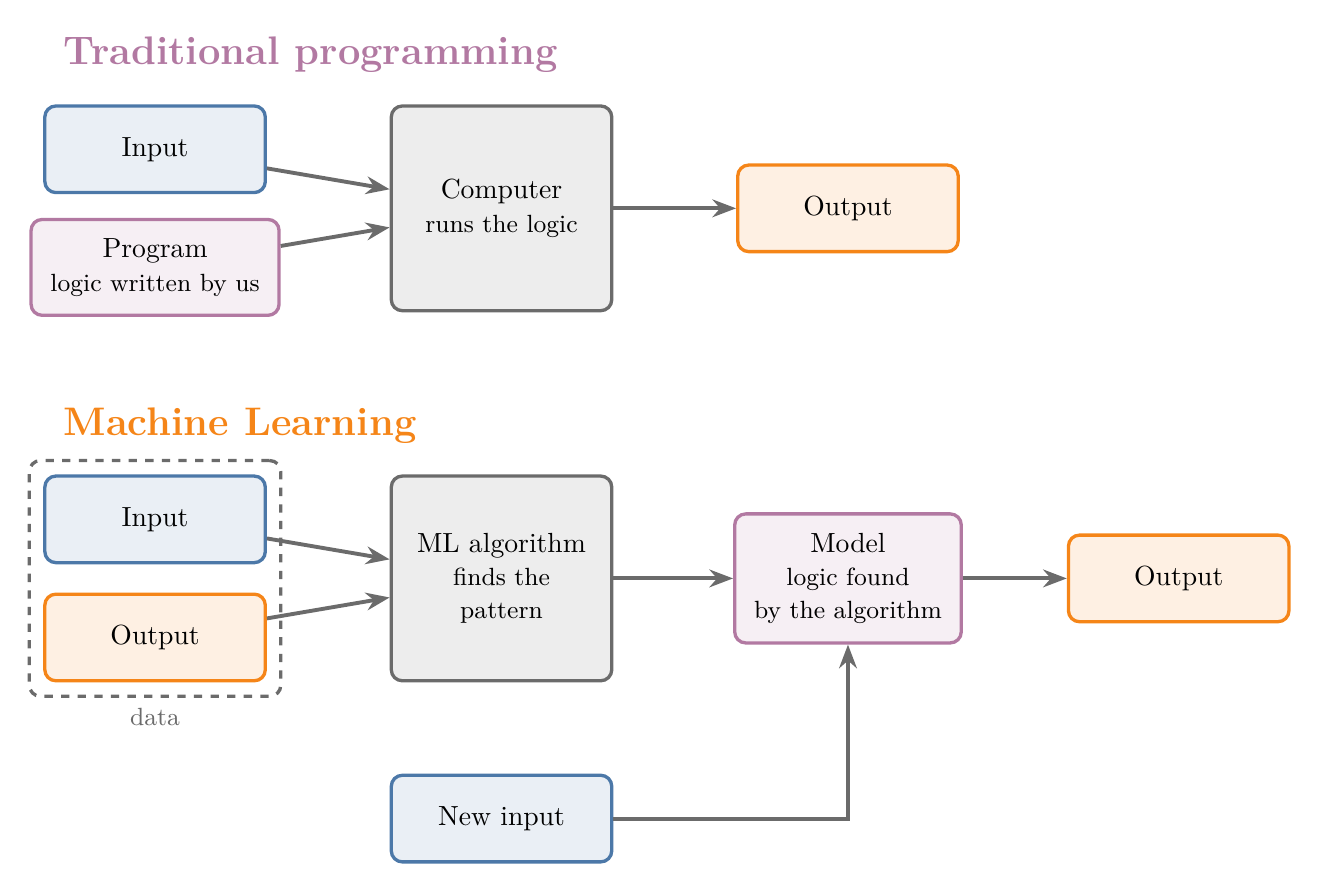
\begin{tikzpicture}
  % top row: traditional programming
  \node[title, cpurple, anchor=west] at (-1.3,3.1) {Traditional programming};
  \node[box=cblue, minimum width=2.8cm] (i1) at (0,1.9) {Input};
  \node[box=cpurple, minimum width=2.8cm] (p1) at (0,0.4) {Program\\{\small logic written by us}};
  \node[box=cgrey, minimum width=2.8cm, minimum height=2.6cm] (c1) at (4.4,1.15) {Computer\\{\small runs the logic}};
  \node[box=corange, minimum width=2.8cm] (o1) at (8.8,1.15) {Output};
  \draw[arrow] (i1) -- (c1); \draw[arrow] (p1) -- (c1); \draw[arrow] (c1) -- (o1);
  % bottom row: machine learning
  \node[title, corange, anchor=west] at (-1.3,-1.6) {Machine Learning};
  \node[box=cblue, minimum width=2.8cm] (i2) at (0,-2.8) {Input};
  \node[box=corange, minimum width=2.8cm] (o2) at (0,-4.3) {Output};
  \node[draw=cgrey, dashed, rounded corners=4pt, fit=(i2)(o2), inner sep=5pt, label={[note]below:data}] {};
  \node[box=cgrey, minimum width=2.8cm, minimum height=2.6cm] (a2) at (4.4,-3.55) {ML algorithm\\{\small finds the}\\{\small pattern}};
  \node[box=cpurple, minimum width=2.8cm] (m2) at (8.8,-3.55) {Model\\{\small logic found}\\{\small by the algorithm}};
  \draw[arrow] (i2) -- (a2); \draw[arrow] (o2) -- (a2); \draw[arrow] (a2) -- (m2);
  % using the model
  \node[box=cblue, minimum width=2.8cm] (n3) at (4.4,-6.6) {New input};
  \node[box=corange, minimum width=2.8cm] (o3) at (13.0,-3.55) {Output};
  \draw[arrow] (n3) -| (m2);
  \draw[arrow] (m2) -- (o3);
\end{tikzpicture}
\end{document}
